% Options for packages loaded elsewhere
\PassOptionsToPackage{unicode}{hyperref}
\PassOptionsToPackage{hyphens}{url}
%
\documentclass[
  12pt,
]{article}
\usepackage{lmodern}
\usepackage{amssymb,amsmath}
\usepackage{graphicx}
\usepackage{ifxetex,ifluatex}
\ifnum 0\ifxetex 1\fi\ifluatex 1\fi=0 % if pdftex
  \usepackage[T1]{fontenc}
  \usepackage[utf8]{inputenc}
  \usepackage{textcomp} % provide euro and other symbols
\else % if luatex or xetex
  \usepackage{unicode-math}
  \defaultfontfeatures{Scale=MatchLowercase}
  \defaultfontfeatures[\rmfamily]{Ligatures=TeX,Scale=1}
  \setmainfont[]{Hoefler Text}
  \setsansfont[]{Gill Sans}
\fi
% Use upquote if available, for straight quotes in verbatim environments
\IfFileExists{upquote.sty}{\usepackage{upquote}}{}
\IfFileExists{microtype.sty}{% use microtype if available
  \usepackage[]{microtype}
  \UseMicrotypeSet[protrusion]{basicmath} % disable protrusion for tt fonts
}{}
\makeatletter
\@ifundefined{KOMAClassName}{% if non-KOMA class
  \IfFileExists{parskip.sty}{%
    \usepackage{parskip}
  }{% else
    \setlength{\parindent}{0pt}
    \setlength{\parskip}{6pt plus 2pt minus 1pt}}
}{% if KOMA class
  \KOMAoptions{parskip=half}}
\makeatother
\usepackage{xcolor}
\IfFileExists{xurl.sty}{\usepackage{xurl}}{} % add URL line breaks if available
\IfFileExists{bookmark.sty}{\usepackage{bookmark}}{\usepackage{hyperref}}
\hypersetup{
  pdftitle={English Department Undergraduate Courses},
  hidelinks,
  pdfcreator={LaTeX via pandoc}}
\urlstyle{same} % disable monospaced font for URLs
\usepackage[paperheight=8.5in,paperwidth=5.5in,bottom=0.75in,top=0.75in,left=0.5in,right=0.5in]{geometry}
\setlength{\emergencystretch}{3em} % prevent overfull lines
\providecommand{\tightlist}{%
  \setlength{\itemsep}{0pt}\setlength{\parskip}{0pt}}
\setcounter{secnumdepth}{-\maxdimen} % remove section numbering
\ifluatex
  \usepackage{selnolig}  % disable illegal ligatures
\fi


\newlength{\cslhangindent}
\setlength{\cslhangindent}{1.5em}
\newlength{\csllabelwidth}
\setlength{\csllabelwidth}{3em}
\newlength{\cslentryspacingunit} % times entry-spacing
\setlength{\cslentryspacingunit}{\parskip}
\newenvironment{CSLReferences}[2] % #1 hanging-ident, #2 entry spacing
 {% don't indent paragraphs
  \setlength{\parindent}{0pt}
  % turn on hanging indent if param 1 is 1
  \ifodd #1
  \let\oldpar\par
  \def\par{\hangindent=\cslhangindent\oldpar}
  \fi
  % set entry spacing
  \setlength{\parskip}{#2\cslentryspacingunit}
 }%
 {}
\usepackage{calc}
\newcommand{\CSLBlock}[1]{#1\hfill\break}
\newcommand{\CSLLeftMargin}[1]{\parbox[t]{\csllabelwidth}{#1}}
\newcommand{\CSLRightInline}[1]{\parbox[t]{\linewidth - \csllabelwidth}{#1}\break}
\newcommand{\CSLIndent}[1]{\hspace{\cslhangindent}#1}

\usepackage{multicol}


\title{Are Large Language Models Operationalizations of Saussurean
Structure?}
\author{}
\date{2022-07-18}

\begin{document}

The title's a bit ugly, but it captures the question I'm trying to ask:
can various computational representations of language/meaning be
usefully understood as ``operationalizations'' of what Ferdinand de
Saussure describes as structure or \emph{langue} in the \emph{Course in
General Linguistics} (1916). Given Saussure's influence in literary
theory and the humanities more broadly,{I leave aside entirely
Saussure's impact in \emph{linguistics}, though my sense is that
Saussure was more put aside than superseded in linguistics. Insofar as
computational approaches to language over the last twenty years
represent something like a turn away from the dominance of Chomskyan
grammar in the second half of the twentieth century, and towards
something grounded in statistics, Saussure does seem a fitting figure.}
I think this would be a useful way of enabling thinking about
computational representations of meaning, from word embeddings (about
which I'll say more) to ``large language models'' and related
technologies that have been kind of amazing to watch develop over the
last year (I'm thinking of GPT-3, of DALL-E\ldots{} all those kind of
jaw dropping pictures circulating on twitter over the past few months).

I'm writing to see if this observation 1) is true, and 2) is useful.
(I'm more uncertain of the latter than the former.) It seems to me that
Saussure's account of language and meaning is a useful analogue to
computational models of meaning because it describes meaning as
\textbf{essentially differential}. (Or, in a Derridean vein,
\emph{différantial}? \ldots{} I want LLMs to bring theory back! Which is
what Ted Underwood predicted\ldots{}
\href{https://tedunderwood.com/2013/08/04/interesting-times-for-literary-theory/}{nearly
a \emph{decade} ago}!) For instance, in trying to explain models like
DALL-E to someone the other day, I was asked: ``So, does it {[}DALL-E{]}
invent something new, or just recombine things from the
internet?''{Underwood captures a version of this in a
\href{https://twitter.com/Ted_Underwood/status/1512813693049917441}{mini-thread
invoking Coleridge's distinction between fancy and imagination from the
\emph{Biographia Literaria}}.} This question captures the challenge of
thinking about, and thinking through, these models. I don't think such
models really do either; they don't spontaneously create new images
\emph{ex nihilo} nor do they simply remix the already existing. But of
course, this binary (creation/recombination) seems an impoverished way
of thinking about how a human generates a text. The rather long and
extensive, and now decades old, tradition of thinking about elements of
culture through Saussure offers a valuable way out of this impasse. This
very question was equally at stake in such (post)structuralist slogans
as Roland Barthes's insistence that ``it is language which speaks, not
the author'' (Barthes 143) (a connection Underwood has also made
\href{https://twitter.com/Ted_Underwood/status/1536681676125913088}{{[}cite{]}}).
At the very least, thinking about these models as Saussurean structures
(rather than as, say, \emph{intelligences}) can forestall some of the
\href{https://www.washingtonpost.com/technology/2022/06/11/google-ai-lamda-blake-lemoine/}{worst
ways} of trying to understand what these models output.

The structuralist overtones of much computationally-driven cultural work
has often come in a Lévi-Straussian flavor, mixed with a desire for a
more empirically grounded work. But that is, I think, only one half
(and, I think, the less influential half) of how structuralism, and the
``theory moment,'' shaped literary theory (to stick to the area with
which I'm most familiar). Returning to Saussure gives an opportunity to
enrich and complicate the structuralist/computational connection. I want
to suggest that these models offer an opportunity to highlight the
essentially \emph{quantitative} element that underlies Saussure and,
indeed, remains implicit in much post-Saussurean and poststructuralist
thinking. This quantitative element is essential, but largely latent, in
Saussure's description of the arbitrary character of the sign.

I think the broad strokes (and perhaps even the narrow strokes) of the
connections between computational models of language (including ``large
language models'') and structuralism seem like they've been in the ether
for a while. For instance:

Sure, they didn\textquotesingle t want to be proved right \emph{like
this.} But that\textquotesingle s always true of prophecy. Poets and
literary critics are still morally required to take a victory lap for
predicting that "it is language which speaks, not the author."
pic.twitter.com/Exw4VGXGZs

--- Ted Underwood ((\textbf{Ted\_Underwood?})) June 14, 2022

"Lang." does seem better for current AI than "intelligence". But
interesting how "lang." here closer to Saussure\textquotesingle s
"langue" (abstract signifying system) than "parole" (actual utterances).
Isn\textquotesingle t lang used as "foundation" model bc it provides a
useful starterpack signifying system?

--- Ryan Heuser ((\textbf{quadrismegistus?})) May 16, 2022

structuralism is back baby!! https://t.co/60gRTTgBQc

--- Robin Manley ((\textbf{\_robinmanley?})) April 26, 2022

These tweets all to some extent express the idea that there is something
about language models/neural networks/``artificial intelligence'' that
recalls structuralism. Bernard Dionysus Geohegan's work on cybernetics
and structuralism and his forthcoming book
\href{https://www.dukeupress.edu/code}{\emph{Code: From Information
Theory to French Theory}} promises to enrich the deeper history of this
connection; but I want to focus on something far more modest.

Indeed, I started this post originally to talk about something much
narrower---J. R. Firth, and the theorization of word embedding vectors.

\hypertarget{on-j.-r.-firth-as-theoretical-inspiration-for-word-embedding-vectors}{%
\subsection{On J. R. Firth as Theoretical Inspiration for Word Embedding
Vectors}\label{on-j.-r.-firth-as-theoretical-inspiration-for-word-embedding-vectors}}

Word embeddings, or word embedding vectors (among other methods), are a
way of representing the meaning of a word with a series of numbers. The
basic idea of word embeddings is to treat a word as a point in
(multidimensional) ``space.''{Listen, writing about these things means
going out on a limb. If there is something grossly wrong this summary,
let me know.} A word's position in space reflects, or represents, its
meaning. Most simply: words with similar meanings should be grouped
together in the same space. \emph{Schnauzers}, \emph{bulldogs}, and
\emph{poodles} might all be constellated around \emph{dog}. A lovely
idea, right? But how to do it?
(\href{https://ryanheuser.org/word-vectors/}{Ryan Heuser's posts on word
vectors} were an invaluable resource when I first read them.)

Key techniques for generating these vectors \emph{embed} a word in this
``semantic'' space by looking at the terms that surround it. If you had
a massive dataset and looked at the words that appear ``near'' (say,
within 2 or 3 words) the terms for dog breeds I just mentioned, you
would find terms for the sort of things dogs do---wag tails, fetch
bones, mark territory, prick up their ears, get dewormed, and so
on.\footnote{These sorts of intuitions---our sense of what terms are
  likely to be near the word ``dog'', for example---crop up frequently
  in discussions of these methods. They offer useful ``just so'' stories
  that inspire these methods; yet it is not clear to me that these
  useful examples are true. We know that dogs do all those things I
  mentioned---but a quick look at the 296 times the term ``dog'' appears
  in the English texts in Andrew Piper's
  \href{https://txtlab.org/2016/01/txtlab450-a-data-set-of-multilingual-novels-for-teaching-and-research/}{txtLab450}
  doesn't show any of those things. In those 296 references, within a
  small window of nearby terms, a dog wags its tail only once; never
  does a dog fetch. Dogs twice dig up bones (though only metaphorical
  dogs, digging metaphorical bones). My point is simply that as we
  reason about how these sorts of methods work, we often rely upon some
  reasonable intuition. Yet those reasonable intuitions don't always
  seem to be supported by the method, and may paper over how genuinely
  alien these methods are to our basic intuitions.} Now we can use those
terms to generate the coordinates for each of our dog-related terms.
Since words with similar meanings have similar collocates, this should
get us our space, right? Carrying this intuition further, we would
assume that \emph{cat} as a term will not be closer in this space to
\emph{bulldog} or \emph{schaunzer} than both of those terms will be to
\emph{dog}. But cat will be closer to \emph{dog} (and any other words in
that ``neighborhood'') than it is to say ``Constitution'' or ``fascism''
(to pick two words chosen entirely without regard to contemporary events
here in the summer of 2022).

From collocation of words to locations of vectors---that's the idea.{All
fine for the English professor to say; but transforming collocation
counts into a meaningful representation is going to involve some linear
algebra.} When people were first oohing and aahing over these things
(back in 2015), one could use some relatively straightforward vector
algebra to do things like querying for the resulting term if one started
with the position of \emph{king}, subtracted the embedding vector
representing \emph{man}, and added in the vector for \emph{woman}.
\texttt{king\ -\ man\ +\ queen} produced, \texttt{queen}, which is
pretty impressive\ldots{} or, it was in 2015. (Compared to the outputs
of DALL-E and GPT-3, this all seems wonderfully quaint.)\footnote{And
  that example seems carefully chosen. Following
  \href{https://douglasduhaime.com/posts/clustering-semantic-vectors.html}{Douglas
  Duhaime's helpful tips}, and this
  \href{https://medium.com/analytics-vidhya/basics-of-using-pre-trained-glove-vectors-in-python-d38905f356db}{medium
  post}, we can easily reproduce it. But my dog examples \emph{do not}
  work. If we try something the words nearest the vector produced
  \texttt{bulldog\ -\ dog\ +\ cat} we get:
  \texttt{\textquotesingle{}cat\textquotesingle{},\ \textquotesingle{}myoot\textquotesingle{},\ \textquotesingle{}bohld\textquotesingle{},\ \textquotesingle{}js04bb\textquotesingle{},\ \textquotesingle{}kahrd\textquotesingle{},\ \textquotesingle{}kd96\textquotesingle{},\ \textquotesingle{}rw95\textquotesingle{},\ \textquotesingle{}greg.wilcoxdailynews.com\textquotesingle{}},
  so\ldots{} yeah.}

In reading the literature about word embedding vectors, the most
frequently cited theoretical inspiration for this approach to meaning is
the British linguistic J. R. Firth. He is quoted with great frequency
for asserting that ``You shall know a word by the company it keeps!'' in
``A Synopsis of Linguistic Theory'' (179).{This essay can be a bit
tricky to track down. If you'd like a PDF, email/DM me.} Firth insists
that meaning be grounded in a ``context of situation,'' a concept that
sounds vaguely related to the ``company {[}a word{]} keeps,'' but the
former is a much broader idea. And for all the citations Firth gets as
inspiration for semantic word vectors, they seem rather far afield of
Firth's central preoccupations in ``A Synopsis.'' Indeed, reading beyond
this passage, one finds very little to help you reason about
collocations quantitatively.\footnote{Anyone looking for the full
  context of the original quote. Here it is, including an interesting
  invocation of Wittgenstein:

  \begin{quote}
  The \emph{placing} of a \emph{text} as a constituent in a context of
  situation contributes to the statement of meanign since situations are
  set up to recognize \emph{use}. As Wittgenstein says, ``the meaning of
  words lies in tehir use.'' The day-to-day practice of palying language
  games recognizes customs and rules. It follows that a text in such
  established usage may contain sentences such as `Don't be an ass!',
  `You silly ass!', `What an ass he is!' In these examples the word
  \emph{ass} is in familiar and habitual company, commonly collocated
  with \emph{you silly---}, \emph{he is a silly---}, \emph{don't be such
  an---}. You shall know a word by the company it keeps! One of the
  meanings of \emph{ass} is its habitual collocation with such other
  words as those quoted. Though Wittgenstein was dealing with another
  problem, he also recognizes the plain face-value, the physiogonomy of
  words. `The sentence is composed of the words and that is enough.'
  (Firth 179).{]}
  \end{quote}}

Firth, in short, provides only the thinnest veneer of theoretical
justification for what word embeddings are, and how they work. An essay
by Mikael Brunila and Jack LaViolette
(\href{https://arxiv.org/abs/2205.07750}{a May 2022 preprint})
summarizes this situation well, discussing J. R. Firth alongside Zelig
Harris as the theoretical inspirations for word embeddings. As they
note, in the word embedding literature ``despite an explosion of
citations\ldots{} this interest {[}in Firth{]} has not been very
engaged.'' Rather, Firth has been invoked in order to ``lend theoretical
authority to a field that struggles to lift its gaze from the latest
state-of-the-art numbers'' (Brunila and LaViolette). If you come to
Firth from discussions of word embeddings (as I did), you may feel
rather puzzled (as I did!), looking (in vain!) for collocation
calculations among talk of ``context of situation'' and the occasional
citation of Alfred North Whitehead (!).

The reason Firth's thinking, or at least Firth's slogan that meaning is
related to the ``company {[}a word{]} keeps,'' is so often cited is
because the technique used by
\href{https://code.google.com/archive/p/word2vec/}{word2vec}, one of the
most influential word embedding models, uses a small window of
collocates to generate its vectors. But this window is more a detail of
implementation, rather than an essential element in how one might
imagine word embedding models (indeed, other word embeddings---including
\href{https://nlp.stanford.edu/projects/glove/}{GloVe}, unless I'm
mistaken, don't use this window). If the core insight of word vectors is
to imagine \emph{meaning} as a point in large dimensional space, then
Firth may not be the most useful theoretical inspiration. The space
these models create is generated by representing a term not simply in
relation to its collocates, but also in relation to all the terms in the
vocabulary. The collocates embed a term in a space that is generated
(originally) by all the terms in the model's vocabulary. It is the sum
total of all the terms that are used, and then how they used in relation
to one another, that really allows meaning to be represented and mapped
in this spatial way.\footnote{Key to word embeddings is reducing the
  dimensionality of this representation. This means that a set of texts
  which may feature a vocabulary in the hundreds of thousands (or
  greater!) can be represented with a ``mere'' few hundred dimensions
  (the \href{https://nlp.stanford.edu/projects/glove/}{pretrained GloVe
  embeddings} are offered in 50, 100, 200, and 300 dimension versions).
  Like the most sophisticated language models and image generators (like
  GPT-3, DALL-E), these embeddings are generated (``learned'') using
  neural networks to reduce their dimensionality. A thing I still don't
  understand: if the complete model were computationally tractable,
  would it be superior to using this significantly smaller model? Or, in
  reducing the dimensionality, do these models help make the vectors
  more ``meaningful'' by ``squishing'' things closer together, and so
  making the meaning more apparent to the various ways in which the
  model can be queried?}

So, we're not just talking about ``the company {[}a word{]} keeps,''
we're talking about a method for generating a ``space.'' Yet even
representing meaning as points in \emph{space} is, to some degree a
technical detail (or, perhaps, a metaphor). Trying to imagine what a
300-dimensional word embedding model ``looks like'' is, of course,
impossible.{I recall a rather funny comment somewhere: asked how to
imagine, say, a twelve-dimensional space, a mathematician responded:
``Imagine a three dimensional space. Now concentrate while saying 12
loudly.''} While the algorithms and measures of distance used in such
models have geometrical interpretations that make them easier to
understand, what we're really talking about is not ``space'' as we
(non-mathematicians) visualize or imagine it. Or, we might say, it is
very easy to imagine what a 300-dimensional word embedding looks like:
it looks like a spreadsheet with 300 columns, and rows for each term in
the vocabulary. What these models are quantifying and representing is
not space, but the \emph{differences} among the terms.

So this is my point: if these models are best understood as representing
language (or meaning) as a system of differences, then it is Saussure,
far more than Firth, who provides something like a theoretical
description of this model. A set of word embedding vectors, or indeed
most language models as I (in my inexpert way understand them) look very
much like what Saussure calls ``a system of pure values'' (155).

\hypertarget{saussure}{%
\subsection{Saussure}\label{saussure}}

So, let's talk Saussure for a moment. My goal here is simply to
highlight the (I think) often ignored \emph{quantitative} element that
is implicit in Saussure's model of meaning, in order to ask whether
contemporary, computational language models might be described as
operationalized instances of a Saussurean model of meaning.

Central to Saussure's description of language is a rejection of any
attempt to treat it as a list-like aggregation of names paired with
concepts/ideas. One instead had to treat the system as a whole: ``A
language is a system in which all the elements fit together, and in
which the value of any one element depends on the simultaneous
coexistence of all the others'' (Saussure et al. 159). ``Value'' here is
a slightly slippery term. Saussure calls the exchange of a word for an
idea \emph{meaning}, but the relationship a word has to the rest of the
words in a language its \emph{value}. A value is determined not in the
relationship between a word and the object it names, but in relationship
to the other words within a language/system.

Saussure offers an illuminating example of how \emph{value} differs from
\emph{meaning}:

\begin{quote}
The French word \emph{mouton} may have the same meaning as the English
word \emph{sheep}; but it does not have the same value. There are
various reasons for this, but in particular the fact that the English
word for the meat of this animal, as prepared and served for a meal, is
not \emph{sheep} but \emph{mutton}. The difference in value between
\emph{sheep} and \emph{mouton} hinges on the fact that in English there
is also another word \emph{mutton} for the meat, whereas \emph{mouton}
in French covers both.

In a given a language, all the words which express neighboring ideas
help to define one another's meaning. Each set of synonyms like
\emph{redouter} (`to dread'), \emph{craindre} (`to fear'), \emph{avoir
peur} (`to be afraid') has its particular value only because they strand
in contrast with one another. If \emph{redouter} (`to dread') did not
exist, its content would be shared out among its competitors\ldots{} So
the value of any given word is determined by what other words there are
in that particular area of the vocabulary. (160)
\end{quote}

Values don't pre-exist the system, waiting to be labeled; they are, as
we say, produced by the language. The key I want to highlight, however,
is how strongly this description resonates with word vectors (and, I
think, with computational models of language/meaning more broadly).
Saussure's language here---of a ``neighborhood'' of terms; of a
``particular area of the vocabulary''---anticipates models of meaning as
vector space. Saussure's description here is, I think, a better
description/theorization of word-embedding vectors (and similar models)
than Firth's ``company it keeps'' slogan.

After a discussion of differences in inflection systems and verb tenses
across language (as another example, along the
\emph{mutton}/\emph{mouton} distinction, of how values are produced by
language), Saussure summarizes:

\begin{quote}
In all these cases what we find, instead of \emph{ideas} given in
advance, are \emph{values} emanating from a linguistic system. If we say
that these values correspond to certain concepts, it must be understood
that the concepts in question are purely differential. That is to say
they are concepts defined not positively, in terms of their content, but
negatively by contrast with other items in the same system. What
characterizes each most exactly is being whatever the others are not.
(162).
\end{quote}

This reflects what Saussure articulates as a ``paradoxical principle'':
the doubleness of all values. \textbf{One}: a value can be located
within a system of like/comparable values; \textbf{two}, value can also
be exchanged that for something dissimilar. Saussure's example is money,
which can be compared to other monetary values quantitatively, or
exchanged for some object/commodity. In language a word can be compared
to other like values (i.e.~to other words)---but also ``exchanged'' for
something dissimilar (a concept or an idea). When Saussure articulates
this idea, he simply asserted that comparing words to other words is
somehow akin to the quantitative comparison of one monetary value to
another. Vector-space representations of language, I think we have a
more direct model of what this could actually look like.

\par\begin{figure}\centering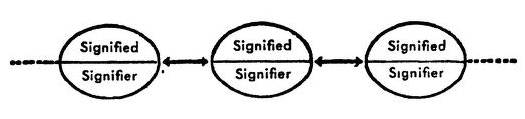
\includegraphics[width=\columnwidth]{_images/saussure_signs.png}\caption{Saussure’s image of a language as a system.}\end{figure}

This crude image of signs relating to one another in a total system
seems to show each term relating only to its neighbors---in a sort of
one dimensional line. But the idea, I take it, is that each term is a
single location within a much larger space, and is defined only by its
difference from all the other terms. Some terms, of course, may be
nearer and further---but the space is defined by all the terms, by the
\emph{langue}.

This understanding of meaning as \emph{differential}, as produced by a
value's (quasi-quantitative) difference from other (quasi-quantiative)
values, is at the heart of---indeed, I'm suggesting it \emph{is the
heart} of---the Saussurean model of meaning. Saussure, of course,
doesn't quantify his values, and doesn't seem to imagine the uses or
benefits of doing so. But the idea of meaning as essentially
differential is, I think, a fundamentally quantitative (even if only
implicitly so) concept.

In the context of intro lit theory classes (of the sort that I teach
with some regularity), I think the stress is sometimes placed on
Saussure's insistence on the arbitrary character of the sign. From this
arbitrariness stems the antifoundationalism that is a hallmark of
poststructuralism. But, for my money (and, probably, Derrida's), it is
the claim that languagef is a system of differences without any positive
values that is the genuinely interesting element of the \emph{Course in
General Linguistics}. After all, the observation that the signifier is
``arbitrary'' is neither novel to Saussure, nor particularly shocking.
Saussure's insight is that if, as seems incontestably obvious, there is
no necessary relationship between what he calls signifier and signified
(a fact well evidenced by the existence of different languages){Saussure
does spend some a brief passage rejecting any attempt to ground meaning
in onomatopoeia (101--02).}, then arbitrary \emph{means} differential:
``the terms \emph{arbitrary} and \emph{differential} designate two
correlative principles'' (Saussure et al. 163). Large language models
represent an operationalization of this idea, they lend calculations to
what was always already (ahem) a quantitative concept.

\hypertarget{so-what}{%
\subsection{So what?}\label{so-what}}

I've contended that Saussure offers a better/richer/more descriptive
theoretical account of word embeddings rather than Firth. But I've
insisted on this point at such length because Saussure also offers a
more recognizable point of reference a wide range of things in the
humanities influenced by structuralism and poststructuralism (the sort
things that folks encounter in humanities classes like ``literary
theory''). If we can recognize large language models are an odd
combination of Saussurean \emph{langue}/\emph{parole}, it seems an
opportunity to leverage a long history of theory in the humanities. Does
Saussure offers a richer point of transit between contemporary
discussions about large language models and the history of theory?

Or, to approach the problem from something like the other dimension:
Does seeing large language models as Saussurean structures reveal a
tacit, quantitative dimension to much structuralist influenced work.
Consider Judith Butler's \emph{Gender Trouble}---certainly one of the
most influential ``theory'' texts. In \emph{Gender Trouble}, Butler
draws a distinction between their own position and structuralism. Butler
writes:

\begin{quote}
The \emph{totality} and \emph{closure} of language is both presumed and
contested within structuralism. Although Saussure understands the
relationship of signifier and signified to be arbitrary, he places the
arbitrary relation within a necessarily complete linguistic system. All
linguistic terms presuppose a linguistic totality of structures, the
entirety of which is presupposed and implicitly recalled for any one
term to bear meaning. This quasi-Liebnizian view, in which language
figures as a systemic totality, effectively suppresses the moment of
difference between signifier and signified, relating and unifying that
moment of arbitrariness within a totalizing field. The poststructuralist
break with Saussure\ldots{} refutes the claim of totality and
universality and the presumption of binary structural oppositions that
implicitly operate to quell the insistent ambiguity and openness of
linguistic and cultural signification. (40)
\end{quote}

This distinction could offer interesting complications to the very of
Saussure I've presented. But what I want to stress is what Butler here
shares with Saussure: a commitment to the arbitrariness of the sign. The
``insistent ambiguity and openness of linguistic cultural
signification'' that is so essential to Butler's larger description of
gender's \emph{performativity}, is not less quantitative/differential
than Saussure's description of \emph{langue}. Such signifying
phenomena---defined by iterability, by arbitrariness, by difference (or
\emph{différance})---imply a differential ``matrix'' (a term used by
poststructuralists and machine learning enthusiasts alike), and so are
in some sense quantitative. I'm \emph{emphatically} not interested in
trying to actually operationalize Butler's account of gender---to attach
numbers to particular gendered signifiers, say---but it seems that
Butler's notion of gender, in desubstantializing gender, makes it
instead an essentially stochastic concept. Perhaps some find that
unsurprising---but this is certainly not the way I'm used to thinking
about gender.

I also think the differences between Saussurean structure and large
language models can be potentially revealing. Saussure infamously
insists on a rigid distinction between the abstract system that a
language constitutes (\emph{langue}) and any particular use/event of
that system (speech or \emph{parole}). The structuralist, in Saussure's
description, studies \emph{langue}, a synchronic system imagined outside
of its history, rather than any particular use or \emph{parole}. While a
vector-space model of meaning (like word embeddings) operates like
\emph{langue}, it is built entirely out of \emph{parole}. These models
scoop up massive amounts of text in order to transform what Saussure
calls \emph{values} into actual numeric values. How should we understand
the implications of this difference? Can we understand issues of
embedded bias
\href{https://nyupress.org/9781479837243/algorithms-of-oppression/}{described
by Safiya Noble}, for instance, as a consequence of treating
\emph{parole} as \emph{langue}? Does such a redescription enable our
thinking in any productive way?

Finally, Saussure reminds us of the inherently social location of the
``intelligence'' these models are able to achieve. If these models
present us with uncanny images of apparent intelligence, it is useful to
recall that the very ``structure'' that these models manage to boil down
and concentrate from so many instances of \emph{parole} is an
intelligence that we have collectively put there. David Weinberger
famously insisted, in what became a sort of slogan for mid 2010s-among
social network enthusiasm, that ``the smartest person in the room is the
room.'' It's a description of the power of networked culture. But, of
course, a room is never ``the smartest person'' ``in the room''; a room
is neither smart nor a person. Weinberger's eminently reasonable
point---(crudely: that people working together have more intelligence
than any individual and that networks enrich/enable this)---is fair
enough, and well taken! The danger is to localize and attribute this
outcome of social organization to a particular technology (here, ``the
room'').{(See also Jerome McGann, \emph{A New Republic of Letters}, pg.
43).} In discussions of language models, I think we sometimes see
something similar---a misattribution of collective, cultural
``knowledge''/``intelligence'' (of the sort that is embedded in language
use) to the particular mechanism/technology for extracting/re-presenting
that intelligence. A crude analogy: a pressure cook can make a mighty
stock, but the flavor comes from the ingredients, not the pressure
cooker. I'm inclined to see Saussure's model of meaning as helping to
remind us that what looks like ``intelligence'' in these models is a
system of relationships that inheres in the material they're trained on.
It is the position of the points that is the source of the word
embeddings power, and that position reflects how the words are used. The
embeddings, or other technologies, can reveal some surprising and
shocking and impressive things; they are truly remarkable. But it is the
system of differences---or the odd pieces of it that are carved off and
thrown into the flow of GPU-powered tensors---which is the location of
the ``intelligence'' such models achieve, far more than than the models
themselves.

\hypertarget{works-cited}{%
\subsection*{Works Cited}\label{works-cited}}
\addcontentsline{toc}{subsection}{Works Cited}

\hypertarget{refs}{}
\begin{CSLReferences}{1}{0}
\leavevmode\vadjust pre{\hypertarget{ref-barthes_death_1977}{}}%
Barthes, Roland. {``The {Death} of the {Author}.''} \emph{Image,
{Music}, {Text}}, translated by Stephen Heath, {Hill and Wang}, 1977,
pp. 142--48.

\leavevmode\vadjust pre{\hypertarget{ref-brunila_what_2022}{}}%
Brunila, Mikael, and Jack LaViolette. \emph{What Company Do Words Keep?
{Revisiting} the Distributional Semantics of {J}.{R}. {Firth} \& {Zellig
Harris}}. arXiv:2205.07750, {arXiv}, 16 May 2022,
\url{https://doi.org/10.48550/arXiv.2205.07750}.

\leavevmode\vadjust pre{\hypertarget{ref-butler_gender_1990}{}}%
Butler, Judith. \emph{Gender {Trouble}: {Feminism} and the {Subversion}
of {Identity}}. {Routledge}, 1990.

\leavevmode\vadjust pre{\hypertarget{ref-firth_synopsis_1968}{}}%
Firth, J. R. {``A Synopsis of Linguistic Theory, 1930-55.''}
\emph{Selected {Papers} of {J}. {R}. {Firth} 1952-59}, edited by F. R.
Palmer, {Indiana University Press}, 1968, pp. 168--205.

\leavevmode\vadjust pre{\hypertarget{ref-saussure_course_1986}{}}%
Saussure, Ferdinand de, et al. \emph{Course in general linguistics}.
{Open Court}, 1986.

\end{CSLReferences}

\end{document}
